\documentclass[11pt]{article}
\usepackage[a4paper,margin=1 in]{geometry}
\usepackage{graphicx}
\usepackage{caption}
\usepackage{subcaption}
\usepackage{listings}
\begin{document}

\title{Calculator using Arduino,LCD \& Push Buttons}
\author{R Rohith Reddy}
\date{\today}
\maketitle


\section{Objective}
	To make a simple calculator using Arduino where input is given through 4x4 keypad made of push buttons and display the whole operation on a 16x2 LCD display.
\section{Components Required}
\begin{enumerate}
 	\item Resistor-220Ohm
 	\item Arduino Uno board
 	\item 16x2 LCD display
 	\item 16 Push buttons
 	\item Jumper wires
\end{enumerate}

\section{Introduction}
	\subsection{Arduino UNO}
		The Arduino UNO is an open-source microcontroller board based on the Microchip ATmega328P microcontroller and developed by Arduino.cc.The board is equipped with sets of digital and analog input/output (I/O) pins that may be interfaced to various expansion boards (shields) and other circuits.The board has 14 Digital pins, 6 Analog pins, and programmable with the Arduino IDE (Integrated Development Environment) via a type B USB cable.
	\subsection{4x4 Keypad}	
		A keypad is a set of buttons arranged in a block or pad which bear digits, symbols or alphabetical letters.The 4*4 matrix keypad usually is used as input in a project. It has 16 keys in total, which means the same input values.
\begin{figure}[h]
	\begin{minipage}[b]{.5\linewidth}
		\centering
		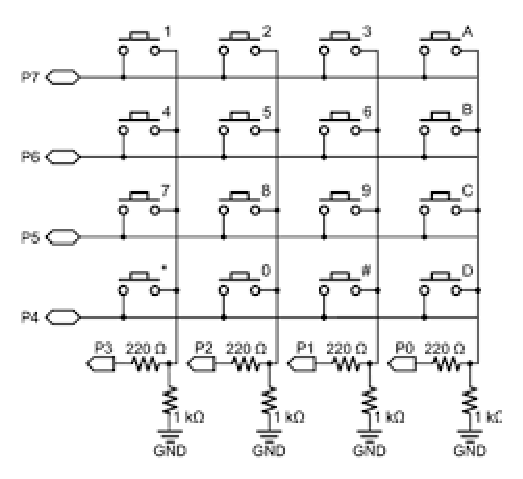
\includegraphics[scale=1]{4x4}
		\caption{ 4x4 keypad matrix using push buttons}
		\label{fig:1}
	\end{minipage}
  	\hspace{0.5cm}	
	\begin{minipage}[b]{.5\linewidth}
		\centering
		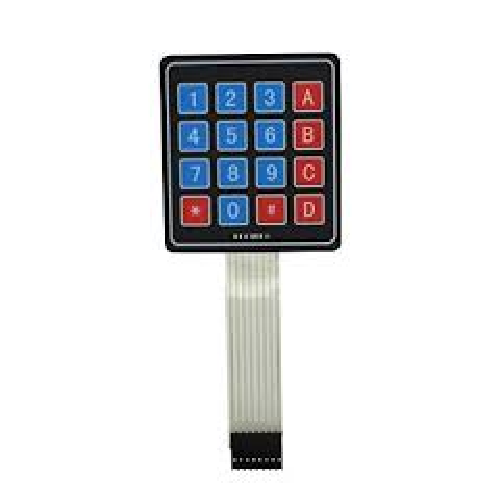
\includegraphics[scale=0.85]{keypad}
		\caption{4x4 Keypad}
		\label{fig:1}  
		\end{minipage}
\end{figure}

	\subsection{16x2 LCD}
		LCD (Liquid Crystal Display) screen is an electronic display module and find a wide range of applications.A 16x2 LCD means it can display 16 characters per line and there are 2 such lines. In this LCD each character is displayed in 5x7 pixel matrix.
		
\section{Hardware Setup}
		\subsection{Push buttons to Arduino connections}
		\begin{enumerate}
			\item Connect the 16 push buttons on the bread board in a 4x4 matrix type and assume a value for each push button.
			\item Using connecting wires/jumpers connect the 16 push buttons as shown in the Figure 1.
			\item Connect the column wires to D0,D1,D6,D7 pins of aurdino and the row wires to D8,D9,D10,D13 of the arduino.
			\item Note:In this calculator the push buttons are given following values/characters:
			\begin{table}[h]
			\centering
			\begin{tabular}{llll}
			'0'   '1'   '2'   '3' \\
			\\
			'4'   '5'   '6'   '7' \\
			\\
			'8'   '9'   '='   '.' \\
			\\
			'+'   '-'   '*'   '/'
			
			\end{tabular}
			\end{table}
			
	\end{enumerate}
	\subsection{LCD to Arduino connections}
		\begin{enumerate}
		\item Connect the 5V pin of the Arduino to an extreme pin of the Breadboard shown in Fig. 1. Let this pin be Vcc.
		\item Connect the GND pin of the Arduino to the opposite extreme pin of the Breadboard.
		\item Connect the arduino to the computer so that it is powered.
\begin{figure}[h]
	\begin{minipage}[t]{.5\linewidth}
		\centering
		\vspace{-5.5cm}
		\includegraphics[scale=1]{lcd}
		\caption{ LCD pin out}
		\label{fig:1}
	\end{minipage}
  	\hspace{0.5cm}	
	\begin{minipage}[t]{.5\linewidth}
		\centering
		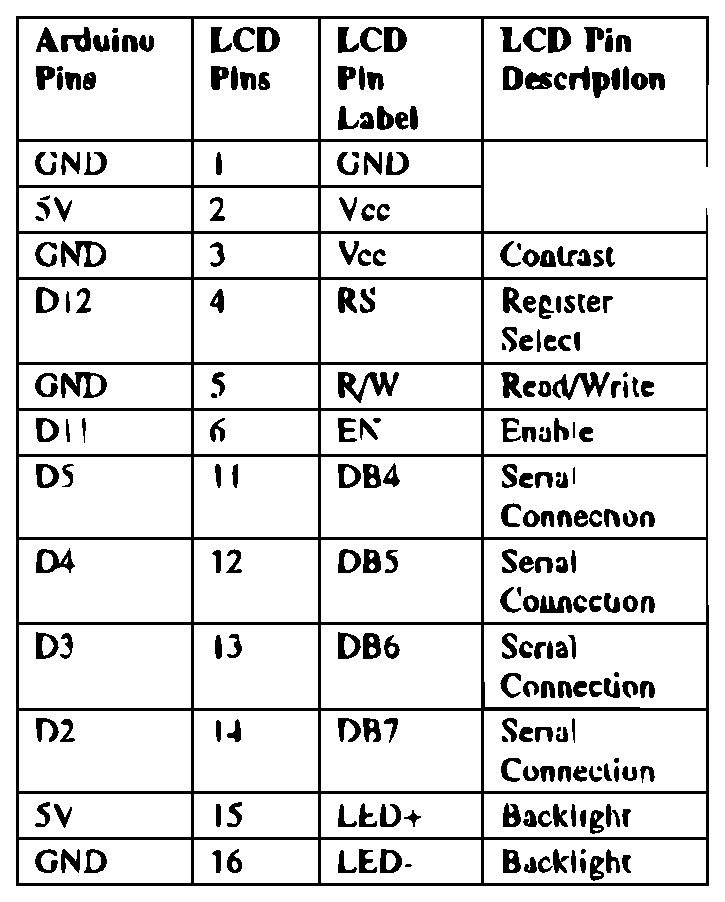
\includegraphics[scale=1]{lcd_connections}
		\caption{ Arduino to LCD Pin Connection}
		\label{fig:1}  
		\end{minipage}
\end{figure}
		
		\item Plug the LCD in Figure 3 to the bread-board.
		\item  Connect the 220$\Omega$ resistance from Vcc to pin 15 (Led+) of the LCD.
		\item Connect the Arduino pins to LCD pins as per Figure 4.
		\end{enumerate}

		
\section{Programming of Arduino}
	Using the arduino IDE write the code for the calculator.The code for the calculator is attached in the appendix H.\\
	The necessary libraries such as Keypad.h and LiquidCrystal.h have to be added to the libraries of the arduino.

\section{Specifications of Calculator}
\begin{enumerate}

	\item Any number of inputs can be given to the calculator with any operations between the operands.
	\item The input can be a decimal number also and  can be a n digit number.
	\item If more than two inputs is given,it performs calculation of first two operands and the obtained result is used for next calculation with third operand and so on.\\
	For example if 2+3*4 is given it first adds 2+3=5 and this 5 is multiplied to 4 and the final result will be shown as 20.
	\item The result of the given input calculation along with the calculation entered is displayed on the LCD display for 4s.After 4s we can enter new calculation.
			
\end{enumerate}

\section{Conclusions}
A simple calculator with basic operations is made using an arduino and push buttons.All 14 digital pins of arduino are used for this purpose.\\
Using C programming we can write code for the calculator by importing certain libraries.
		
\renewcommand\thesection{\Alph{section}}
\section{Appendix}
The arduino code for calculator:
\begin{lstlisting}
#include <Keypad.h>
#include <LiquidCrystal.h>
#include <stdlib.h>

LiquidCrystal lcd(0,1,5,4,3,2);
float result(char [],int );

int i=0,count=0;
char arr[20],data,key,sign[10];
float ans;
const byte ROWS = 4; /* four rows */
const byte COLS = 4; /* four columns */
/* define the symbols on the buttons of the keypads */
char hexaKeys[ROWS][COLS] = {
  {'0','1','2','3'},
  {'4','5','6','7'},
  {'8','9','=','.'},
  {'+','-','*','/'}
};
byte rowPins[ROWS] = {10, 11, 12, 13}; /* connect to the row pinouts of the keypad */
byte colPins[COLS] = {6, 7, 8, 9}; /* connect to the column pinouts of the keypad */

Keypad customKeypad = Keypad( makeKeymap(hexaKeys), rowPins, colPins, ROWS, COLS); 

void setup(){
  lcd.begin (16,2) ; 
  lcd.setCursor (5,0) ;
  lcd.print ("Simple") ;
  lcd.setCursor (3,1) ;
  lcd.print ("Calculator") ;
  delay(1000);
  lcd.clear();
}

void loop(){  
 
char key = customKeypad.getKey();
  
  if (key != NO_KEY && (key=='1'||key=='2'||key=='3'||key=='4'||key=='5'||key=='6'||key=='7'||key=='8'||key=='9'||key=='0'||key == '/' || key == '*' || key == '-' || key == '+'||key=='.'))
  {
    arr[i]=key;
    lcd.setCursor (i,0);
    lcd.print(arr[i]);
    i=i+1;
  }
  if(key=='='){
    arr[i]='=';
    lcd.setCursor (i,0);
    lcd.print(arr[i]);
    ans=result(arr,i+1);
    lcd.setCursor (0,1);
    lcd.print("Result:");
    lcd.print(ans);
    delay(2000);
    i=0;
    lcd.clear();
  }

}


float result(char a[],int len)
{
int i,count,op[10],j=0,k=0,n=0;
float res,h[10];
char num[10][10],sign[10],nw[100],an[100];
count=len;
for(i=0;i<count;i++)
{
  lcd.setCursor (i,0);
   lcd.print(arr[i]);
}
for(i=0;i<count+1;i++)
{
  if(a[i]=='+'||a[i]=='-'||a[i]=='*'||a[i]=='/'||a[i]=='=')
  {
    op[j]=i;
    sign[j]=a[i];
    j=j+1;
  }
} 
for(n=0;n<j;n++)
{ 
  if(n==0)
  {
    for(k=0;k<op[n];k++)
    {
    nw[k]=a[k];
    nw[k+1]='\0';
      h[n]=atof(nw);
    }
  }
  else 
  {
    for(k=0;k<op[n]-op[n-1]-1;k++)
    {
    nw[k]=a[op[n-1]+1+k];
    nw[k+1]='\0';
      h[n]=atof(nw);
    }
  }}    

k=0;
  for(i=0;i<j-1;i++)
  {
    switch(sign[k])
    {
    case '+':
      res=h[i]+h[i+1];
      break;
    case '-':
      res=h[i]-h[i+1];
      break;
    case '*':
      res=h[i]*h[i+1];
      break;
    case '/':
      res=h[i]/h[i+1];
      break;
    }
    h[i+1]=res;
    k=k+1;
  }
return res;
}

\end{lstlisting}
\end{document}